\chapter{Implementation}

At its core, the application is a standard forward rendering engine supporting multiple lights, shadow mapping, and normal mapping---in addition, of course, to full real-time dynamic global illumination. The scene to be rendered is composed of one or more actors, which are simply meshes loaded from the generic Wavefront OBJ file format. Actors are also capable of rigid body animations.

The rendering pipeline can be broken down into several render passes, each of which will be explained in its corresponding section. In general, the main steps taken are generating a voxelized representation of the scene, creating a filtered representation of light from the voxels and light sources, and finally shading the scene.

The application itself is written in C++11 and uses OpenGL as the graphics API. In order to make use of modern graphics features like compute shaders and direct state access we require OpenGL version 4.5 (released in 2014). The project uses CMake as its build system and has been tested on Linux and Windows.

% TODO should I mention conventions used for variables and such?

% TODO using tinyobj w/ http://exocortex.com/blog/extending_wavefront_mtl_to_support_pbr for pbr
% PBR shading (Cook-Torrance, Disney, UE4, ...) https://disney-animation.s3.amazonaws.com/library/s2012_pbs_disney_brdf_notes_v2.pdf

% TODO include code snippets, API calls, diagrams
%TODO name the 3D texture (and refer to it in monospace)?
\section{Voxelization}
The goal of voxelization is to create a sparse 3D representation of the geometry in the scene. The information associated with each voxel is stored in two 3D textures: one for color and opacity and another for surface normal. We refer to these textures as \texttt{voxelColor} and \texttt{voxelNormal}, respectively. Each texture has an internal format of \texttt{RGBA16F} or \texttt{RGBA8}, depending on hardware capabilities. The resolution of the textures are configurable at runtime, although the default is $256^3$.

The extents of our voxelization volume---the area in world space that will end up inside the voxel textures---is also configurable and by default is set to enclose the entire scene. This volume can be static or can track the camera (with the camera being at the center of the textures). In addition, to prevent some issues with temporal artifacts, the voxel textures are snapped to a discrete grid corresponding to the size of each voxel cell in world space.

We present two different approaches for scene voxelization: one utilizing hardware rasterization and the other hardware tessellation.

\subsection{Rasterization-Based Approach to Voxelization}
% TODO scene extents, midpoint and tracking, computing voxel texture coordinates, choosing axis, diagram of scene extents and converting to NDC
% TODO cite GPU Pro 4 and imageAtomicMax
The first method for voxelization implementated utilizes the GPU rasterization pipeline and is based on~\cite{crassin2012octree}. The voxelization is performed completely in a single render pass. The basic idea is to rasterize the scene such that each fragment generated by the GPU corresponds to a single voxel in the 3D texture.
One of the main challenges with voxelization is ensuring there are no holes or cracks in the resulting grid. Two techniques are used to mitigate this (and will be covered in-depth in the following paragraphs). First, for each triangle we project along the triangle's normal's dominant axis. This maximizes the number of fragments generated for a given triangle. Second, we perform conservative rasterization. Normally, the GPU only generates a fragment for a given pixel if a triangle overlaps the center of the corresponding pixel. This results in cracks in the voxelized grid since even if a triangle is inside a voxel it may not be rasterized.

Before the draw call, the necessary matrices to project the geometry into the voxelization volume are created. The projection matrix is orthographic, with bounds corresponding to the extents of the voxelization volume. In order to project along each triangle's dominant axis, we also need three view matrices: for each axis a view matrix is constructed where the view position is at the edge of the voxel volume and looks down its respective axis. The final matrix used to transform a point in world space to a point in the voxel texture for a particular axis is composed by multiplying the orthographic matrix with the appropriate view matrix.

% TODO what do with this
For the shader program, the voxel textures are bound as \texttt{image3D} objects (as textures are read-only in shaders). Following from that, since the framebuffer is not being written to, color writing is disabled. Lastly, depth testing and depth writes are also disabled, since the goal is to voxelize the entire scene. The algorithm is shown in Algorithm~\ref{alg:voxelization} and explained in detail below.

\begin{algorithm}
    \caption{Voxelization}
    \label{alg:voxelization}
    \begin{algorithmic}
        \For {each triangle $t$}
        \State {find dominant axis of $t$ using surface normal}
        \State {apply projection matrix corresponding to the dominant axis}
        \EndFor
        \State{Rasterization}\Comment {Performed by hardware}
        \For {each rasterized fragment} \Comment {position is in NDC}
        \State {transform NDC coordinates to texture space ($[0, 1]$)}
        \State {Realign NDC coordinates with standard coordinate system}
        \State {Insert fragment into voxel texture}
        \EndFor
    \end{algorithmic}
\end{algorithm}

Starting in the vertex shader, the only operation performed is transforming the object from object space to world space using its appropriate model matrix. In the geometry shader we take a single triangle in world space, transform it based on its dominant axis, and output the resulting triangle in clip space. The triangle's dominant axis is determined by finding the largest component of its normal (by absolute value)\footnote{Finding the dominant axis is really finding the maximum dot product of each axis with the normal, but since we use the standard basis this reduces to just finding the largest component of the normal.}. We then apply the appropriate projection matrix according to the dominant axis and output the resulting triangle to be rasterized. In the fragment shader, each fragment's position in Normalized Device Coordinates can be used to determine its position within the voxel textures. Note, however, that the components of each fragment's position need to be realigned due to projecting along different axes. Finally, the voxel information can be written into the voxel textures, which are bound as \texttt{image3D} objects in the shader. The result of this voxelization is shown in Figure~\ref{fig:voxels_off}.

However there is still one more issue: multiple voxel fragments can be mapped to the same cell in the voxel textures. Without any synchronization, the final voxel values are not deterministic and can result in temporal artifacts. To solve this, we average the resulting color value using atomic operations\footnote{Other approaches to this problem (with various tradeoffs) can be used (Doghramachi uses an atomic max operation on a custom defined metric in order to avoid needing to perform an average~\cite{doghramachi2013rasterized}). These are generally used to combat performance issues or hardware limitations.}.
% TODO should explain rgba8 + faking atomic avg vs rgba16f + atomicAdd + compute shader
% TODO 'we implemented both atomicavg and atomicmax and prefer atomicmax for its simplicity, greater reliability, and negligible difference in lighting'

\begin{figure}[h]
\centering
    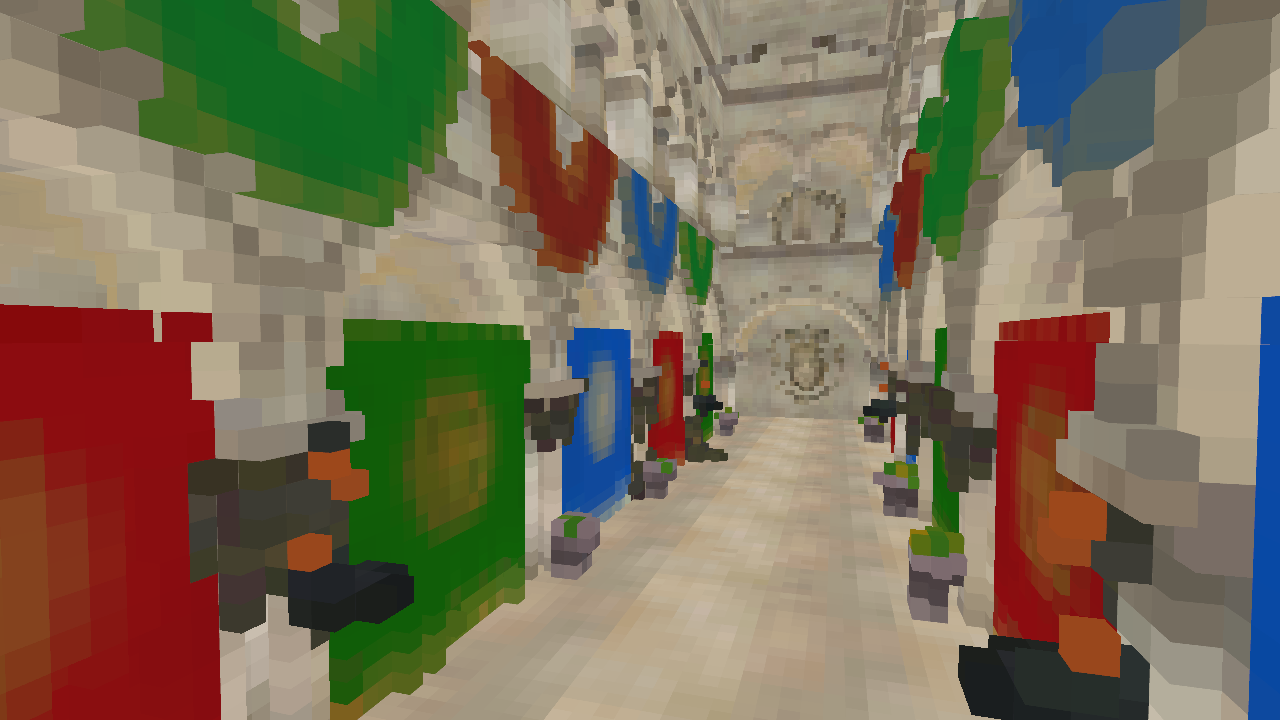
\includegraphics[width=\textwidth]{voxels_off.png}
    \caption{Visualization of the voxels resulting from the rasterization-based approach (without conservative rasterization).}
    \label{fig:voxels_off}
\end{figure}

% TODO need to work this in better. subsection?
% TODO should expand on problem more
\subsubsection{Conservative Rasterization}
As mentioned previously, we need conservative rasterization to minimize holes and cracks in the voxelization. To achieve this, we use an MSAA based approach~\cite{takeshige2015basics}. MSAA (multi-sample anti-aliasing) is a technique used for smoothing out ragged edges (aliasing) in a rasterized image. Instead of only sampling at one position inside a pixel to determine if a fragment should be generated multiple samples are used (hence the name). These samples are typically distributed to maximize the possibility of a rasterized fragment being produced. If any of the samples overlap with the triangle a fragment is generated for that pixel. An illustration of MSAA is shown in Figure~\ref{fig:msaa}. Applied to voxelization, this means there is a smaller chance that a triangle will fail to produce a fragment for any voxel it only partially occupies. While the MSAA method of conservative rasterization is not perfect (a partially occupied voxel won't always produce a fragment), it is cross-platform, simple to use, and efficient. Other notable methods would be manually dilating each triangle in a geometry shader (better quality but slower)~\cite{akenine2005conservative} or using a GPU vendor specific extension, like \verb#GL_NV_conservative_raster# (better quality but not cross-platform). A comparison between no conservative rasterization, MSAA-based conservative rasterization, and the NVIDIA extension is shown in Figure~\ref{fig:conservativerasterization}\footnote{Also note the erroneous fragments generated when using the NVIDIA extension. These extra fragments are produced by some methods of (overly) conservative rasterization and relies on the user to manually cull these fragments.}.

\begin{figure}[h]
    \centering
    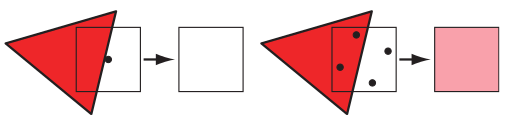
\includegraphics[width=\textwidth]{rtr_fig5_28.png}
    \caption{With MSAA, multiple points within a pixel are used to determine whether a fragment should be generated~\cite{moller2008rtr}.}
    \label{fig:msaa}
\end{figure}

% TODO should implement the geometry shader based and then compare performance quality of all 3 (might need to do that indirect rendering thing too...)

% Camera Position (8.0, 2.7, -1.3), Direction (-1.0, -0.0, 0.3)

\begin{figure}[h!]
\centering
    \begin{subfigure}[t]{0.65\textwidth}
        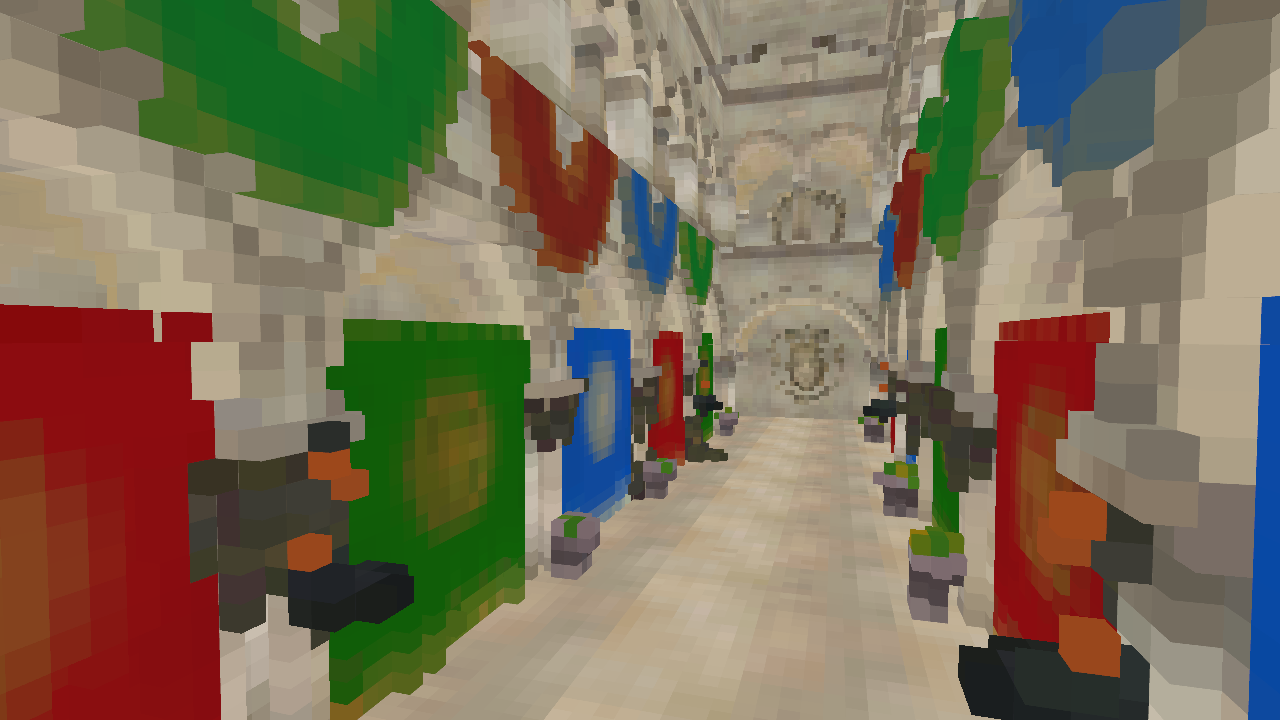
\includegraphics[width=\textwidth]{voxels_off.png}
        \caption{No conservative rasterization}
    \end{subfigure}
    \begin{subfigure}[t]{0.65\textwidth}
        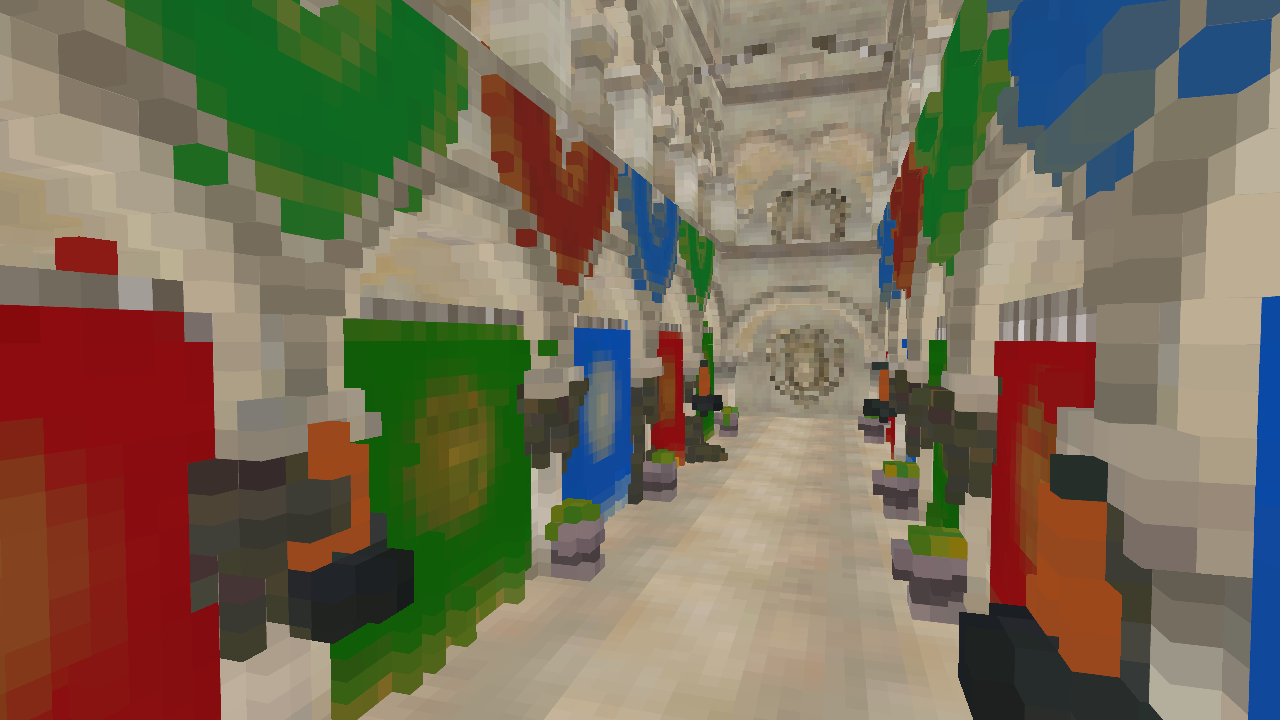
\includegraphics[width=\textwidth]{voxels_msaa.png}
        \caption{MSAA-based conservative rasterization}
    \end{subfigure}
    \begin{subfigure}[t]{0.65\textwidth}
        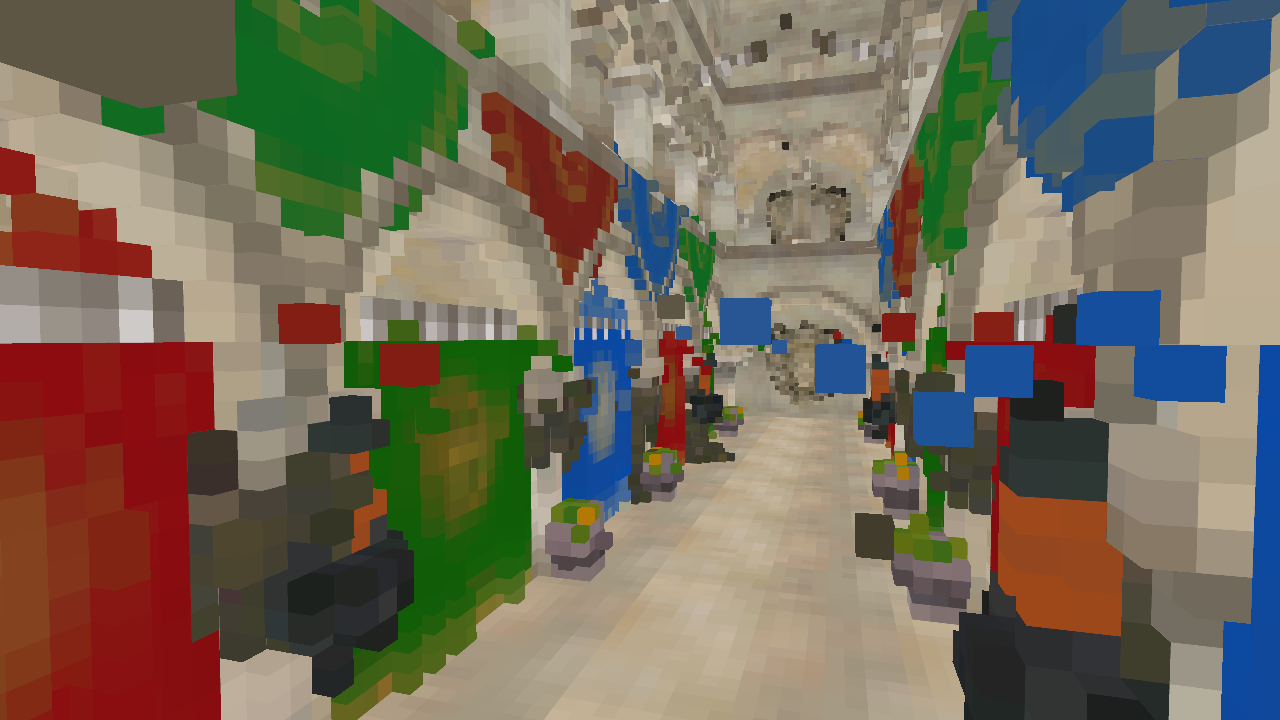
\includegraphics[width=\textwidth]{voxels_nv.png}
        \caption{NVIDIA's conservative rasterization extension}
    \end{subfigure}
    \caption{Conservative rasterization produces `extra' fragments in order to produce a more solid voxelization. The effects are particularly noticeable on the pillar between the red and green curtain on the left.}
    \label{fig:conservativerasterization}
\end{figure}

\subsection{Tessellation-Based Approach to Voxelization}
The other method for voxelization relies completely on hardware tessellation: no rasterization required. Instead of generating fragments for each voxel we instead attempt to generate vertices for each voxel. One benefit of this method is the mapping from vertex to voxel position is fairly straightforward and does not require multiple projection matrices like in the rasterization-based approach. Fei et al.~\cite{Fei:2012:PV:2305276.2305280} also developed an algorithm similar to ours using tessellation.

The core part of this approach is determining the appropriate tessellation level for a given triangle. Recall that this step is the responsibility of the tessellation control shader. Afterwards, tessellation primitive generation produces the tesselated vertices and provides them to the tessellation evaluation shader, where we compute each vertex's position in the voxel texture and store the vertex's color. The final voxelized scene is shown in Figure~\ref{fig:tesselatedvoxels}.

% TODO determining tessellation level and discarding
The desired level of tessellation will produce one vertex for each voxel the triangle covers. Therefore, for a particular triangle, the tessellation level is determined based on the triangle's size in world space. Recall that for triangular tessellation patches there are four values: three outer tessellation levels (one for each edge) and one inner tessellation level. To determine the outer tessellation level for an edge $E$, we effectively determine how many voxels $E$ passes through (accounting for the direction of $E$): $\displaystyle outerLevel = \frac{|E|}{(\frac{E}{||E||} \cdot voxelSize)}$. To determine the inner tessellation level, we find the maximum altitude of the triangle and then perform a similar computation as with the outer level. With $a$, $b$, and $c$ being the lengths of the triangle edges, the altitude from a side $x \in \{a, b, c\}$ is given by
\[
    h_x = \frac{2 \sqrt{s(s-a)(s-b)(s-c)}}{x}
\]
where $s = (a + b + c) / 2$ is the semiperimeter and the square root term is the triangle's area using Heron's Formula. The maximum altitude is then $h_{max} = \max(h_a, h_b, h_c)$. Finally, we have $innerLevel = h_{max} / voxelSize$. % TODO should find direction of h_max and do dot product like outer levels

% TODO calculating coordinates and inserting
After specifying the tessellation levels in the tessellation control shader, tessellation primitive generation produces the vertices that correspond to the voxels. In the tessellation evaluation shader the vertex position (in world space) is used to determine the final voxel position and is written out to the voxel texture.

An important consideration for this method is the maximum tessellation level supported by the hardware. For large triangles it is possible the tessellation will not produce a solid voxelization. A simple way to address this issue is to break large triangles into smaller ones when loading the mesh. Another consideration is for small triangles where all vertices occupy a single voxel. To reduce the number of writes to the voxel texture the contributions of these vertices can be consolidated in the shader into a single operation.

\begin{figure}[h!]
\centering
    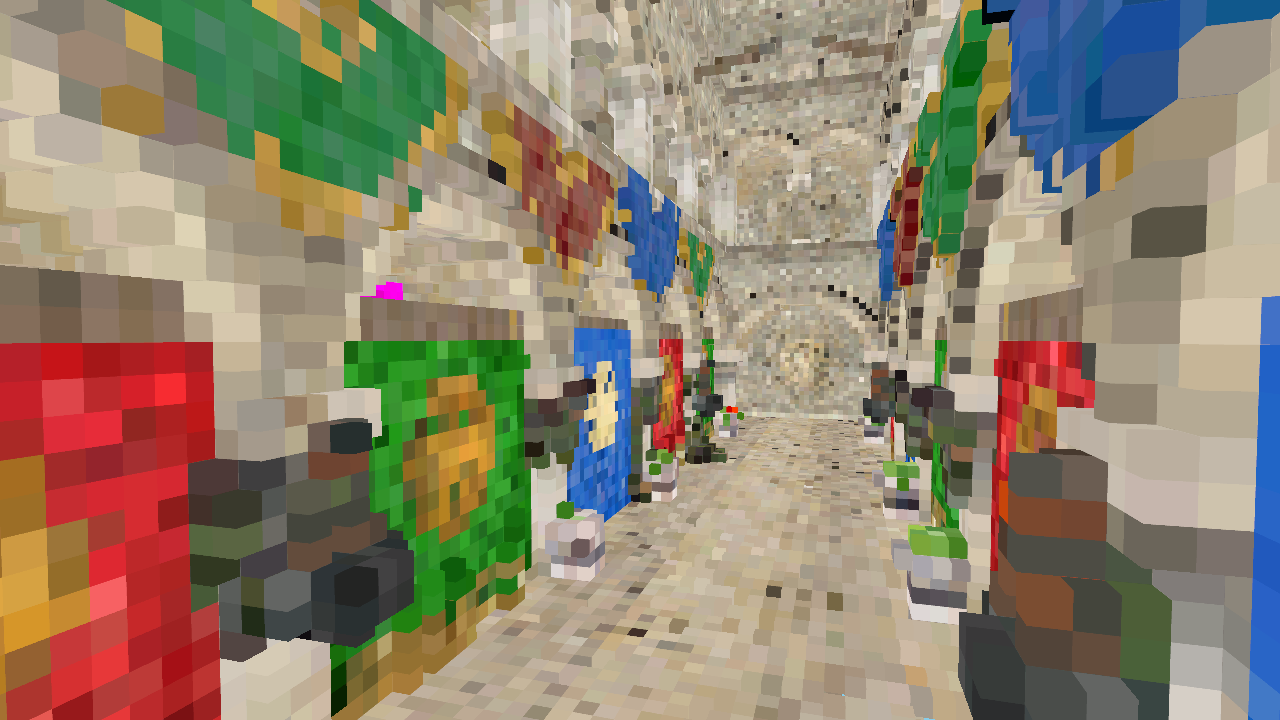
\includegraphics[width=\textwidth]{voxels_tesselated.png}
    \caption{Scene voxelized using tessellation-based voxelization.}
    \label{fig:tesselatedvoxels}
\end{figure}

% TODO code snippets, actual OpenGL names
\section{Shadow Mapping}
Shadow mapping is a well known technique used for efficiently creating shadows~\cite{Williams:1978:CCS:965139.807402}. Similar to the related works, the resulting shadow map is also treated similarly to an RSM for radiance injection.

To generate a shadow map for a light, we render the scene from the light's perspective and gather the depth values of the fragments. Since we need the GPU to write to an arbitrary texture (the shadowmap), we create a framebuffer object (FBO) and attach the texture as a depth attachment\footnote{This general technique is referred to as render-to-texture.}. The FBO does not require any color attachments, as we are only interested in the depth. The matrix used to transform vertices from world space to light space is an orthographic projection matrix multiplied with a view matrix generated from the light. This matrix is often called the light view matrix. Since the GPU will automatically write depth values, the fragment shader can be completely empty. The resulting shadow map contains floating point depth values (in the range [0, 1]) which represent the distance of each point visible to the light to the light itself. Also note that these depth values are linear since an orthographic projection matrix is used: if a perspective projection matrix is used the depth values scale logarithmically. Figure~\ref{fig:shadowmap} shows the contents of a shadowmap for our scene.

The only difference between generating a shadow map and a complete RSM is to also store the diffuse color and normal along with the depth values. Since our implementation stores voxel colors and normals already a full RSM isn't necessary for injecting the VPLs into the radiance texture.

\missingfigure{Possibly show RSM (albedo+normal) too.}
\begin{figure}[h!]
\centering
    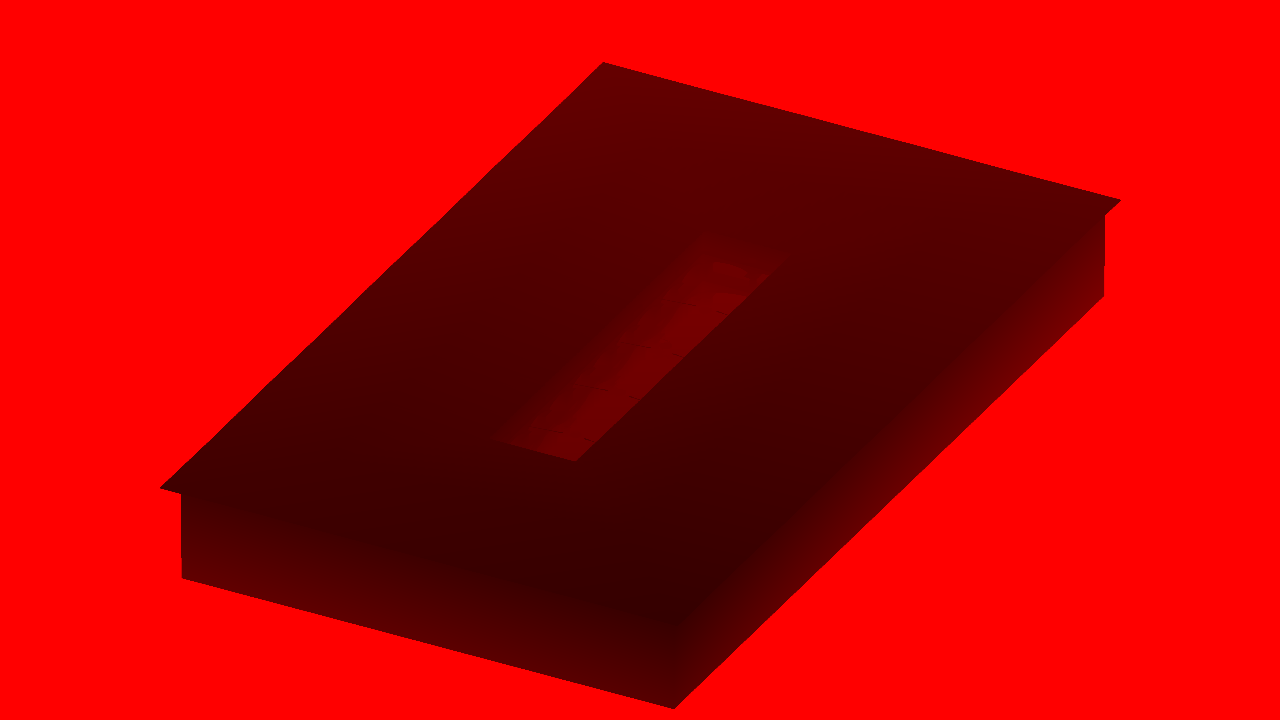
\includegraphics[width=\textwidth]{shadowmap.png}
    \caption{An example of a shadowmap with the depth value mapped to the red component of the image.}
    \label{fig:shadowmap}
\end{figure}

\section{Radiance Injection}
In this render pass, we fill a 3D texture with virtual point lights from the shadow map. Recall that the VPLs are light sources which represent the light being bounced off of geometry within the scene. Following from RSMs, the points at which this happens are precisely where the light hits the geometry, which is stored in the shadow map. Therefore, this pass involves taking all points in the shadow map and projecting the color of the corresponding geometry into the radiance texture.

The radiance texture, \texttt{voxelRadiance}, has dimensions equal to that of the other voxel textures. It has a format of \texttt{RGBA8} and stores a color value and opacity.

The most straightforward way to accomplish radiance injection from the shadow map is to use a compute shader and launch one thread for each pixel in the shadow map. Each thread first reads the depth value at its respective pixel, which can then be used to reconstruct the pixel's position in light space. Then, by using the inverse light view matrix, we project it from light space to world space. The world space position is used to calculate the voxel position, which is used to sample from the voxel textures and finally write the color into the radiance texture, as seen in Figure~\ref{fig:radiance}.

It is important the shadowmap is rendered with a high enough resolution (relative to the voxel texture resolution) to ensure a smooth radiance injection. If the shadowmap resolution is too low, there will be gaps between voxels which cause lighting artifacts. Note also that we do not need to be concerned with synchronization and atomic operations in the case that multiple threads access the same voxel position since we are only interested in the base color.

In addition to injecting the VPLs we also transfer occlusion information (opacity) stored in the completely voxelized scene into the radiance texture. This operation is a straightforward transfer accomplished using another compute shader.

% TODO show lighting artifacts if shadowmap resolution too low
% TODO temporal filtering?

% \begin{lstlisting}[language=C,breaklines=true,basicstyle=\footnotesize\ttfamily]
% vec2 shadowmapTexcoord = vec2(threadId) / vec2(shadowmapSize);
% float shadowmapDepth = texture(shadowmap, shadowmapTexcoord).r;
% vec3 ndc = vec3(shadowmapTexcoord, shadowmapDepth) * 2 - vec3(1);
% vec3 worldPosition = (lsInverse * vec4(ndc, 1)).xyz;
% ivec3 voxelPosition = ivec3(voxelIndex(worldPosition, voxelDim, voxelCenter, voxelMin, voxelMax, warpVoxels));
% \end{lstlisting}

\begin{algorithm}
    \caption{Radiance Injection}
    \label{alg:radianceinjection}
    \begin{algorithmic}
        \For{$\text{each pixel coordinate } p = (p_x,p_y) \text{ in shadowmap}$} \Comment{$p_x, p_y \in [0,1]$}
        \State {$depth = \mathrm{sampleDepthFromShadowmap}(p)$}
        \State {$ndc = (p_x, p_y, depth) * 2 - 1$} \Comment{Convert coordinate to NDC}
        \State {$worldPosition = inverseLight * ndc$}
        \State {$voxelPosition = \mathrm{computeVoxelPosition}(worldPosition)$}
        \EndFor
    \end{algorithmic}
\end{algorithm}

\begin{figure}[h!]
\centering
    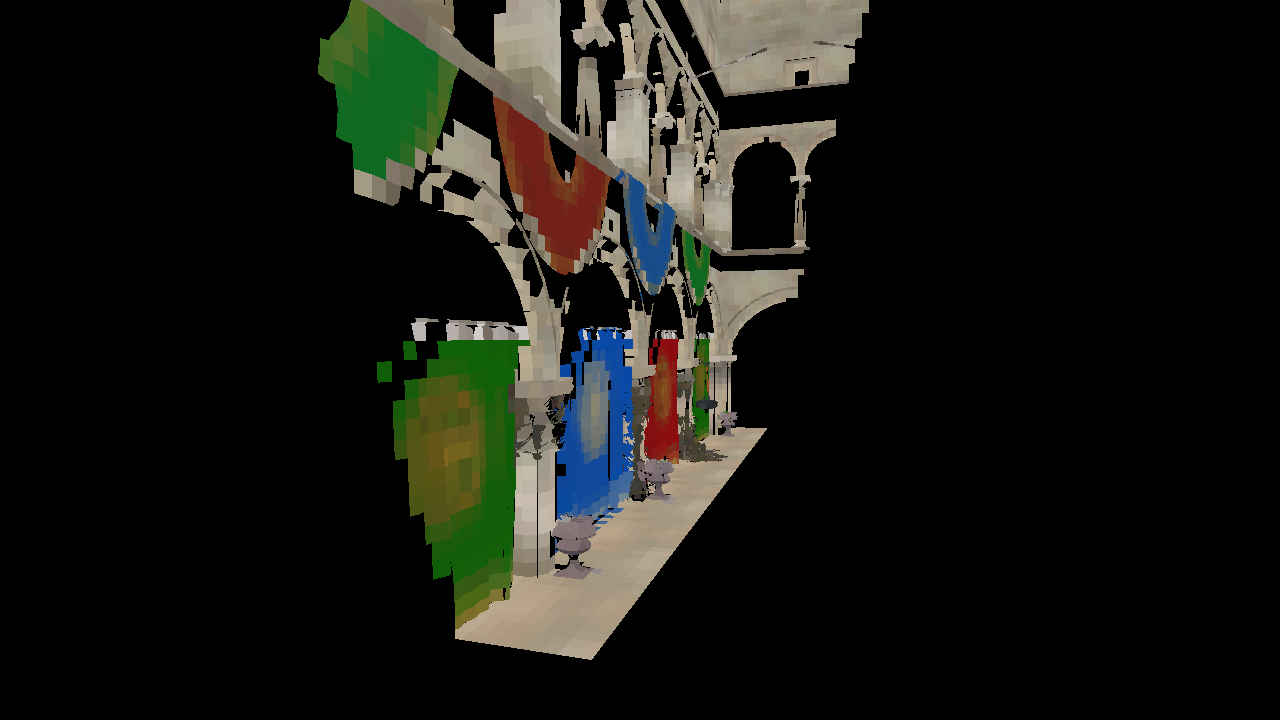
\includegraphics[width=\textwidth]{radiance_nolighting.png}
    \caption{The radiance texture injects VPLs according to the shadowmap: only voxels hit by the light source result in a VPL.}
    \label{fig:radiance}
\end{figure}

\section{Radiance Filtering}
With the highest level of detail of the radiance texture filled, the next step is creating the filtered representation. Each successive level is half the resolution of the previous level. Therefore, the maximum number of levels the texture may have is $log_2 (\max (\text{width}, \text{height})) + 1$.

% TODO timing difference between glgenmipmaps and compute shader
OpenGL is able to automatically generate mipmaps for 3D textures by calling \verb#glGenMipmaps(GL_TEXTURE_3D)#, however manually filtering the textures using a compute shader turned out much faster for this application (how OpenGL calculates mipmaps is implementation defined, so the performance can vary between systems and drivers). To perform the filtering, a compute shader kernel is launched for each level of the radiance texture (not including the base level). The kernel is launched with one thread for each voxel in the current level. Each thread can be conceptually located at the corners of each voxel in the previous level and averages the surrounding 8 values to compute the filtered value of its respective voxel.

% TODO probably remove this, or maybe future work?
The other benefit to manually filtering is different methods can be used. For example, adjusting the size or weights of the filtering kernel could result in different effects.

\begin{figure}[h!]
\centering
    \begin{subfigure}[t]{0.4\textwidth}
        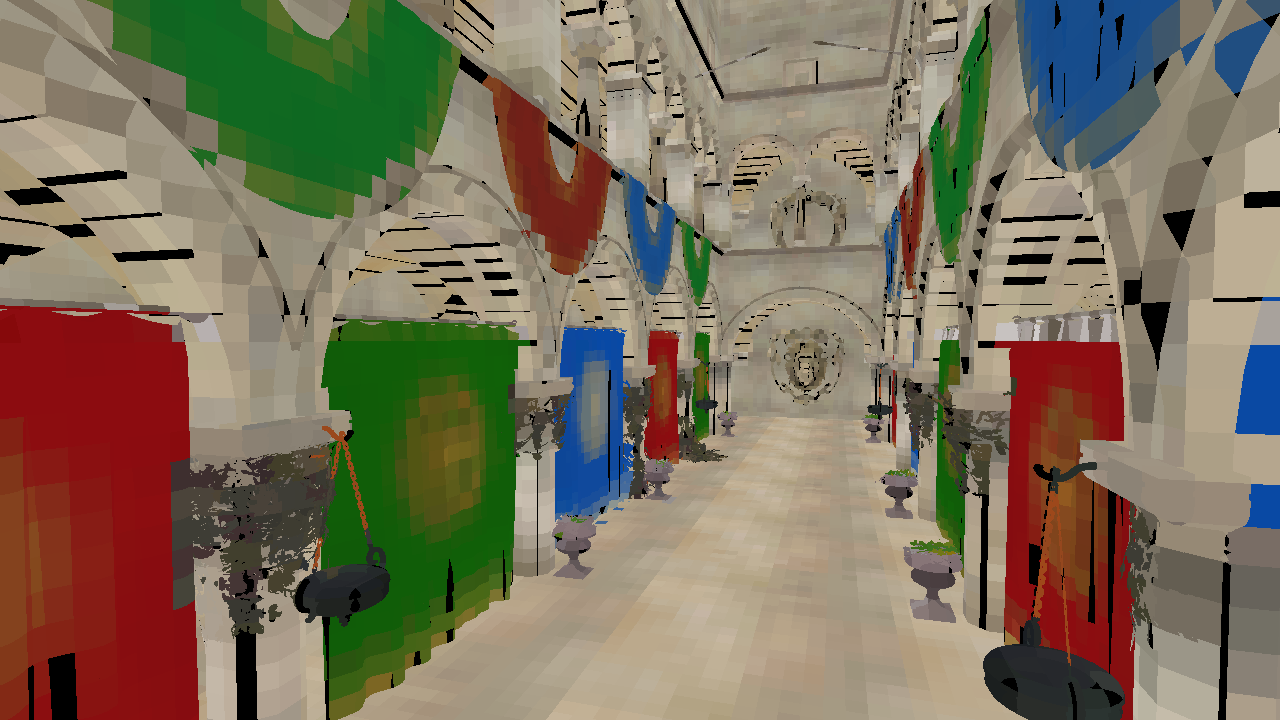
\includegraphics[width=\textwidth]{mipmap0.png}
        \caption{Level 0}
    \end{subfigure}
    ~
    \begin{subfigure}[t]{0.4\textwidth}
        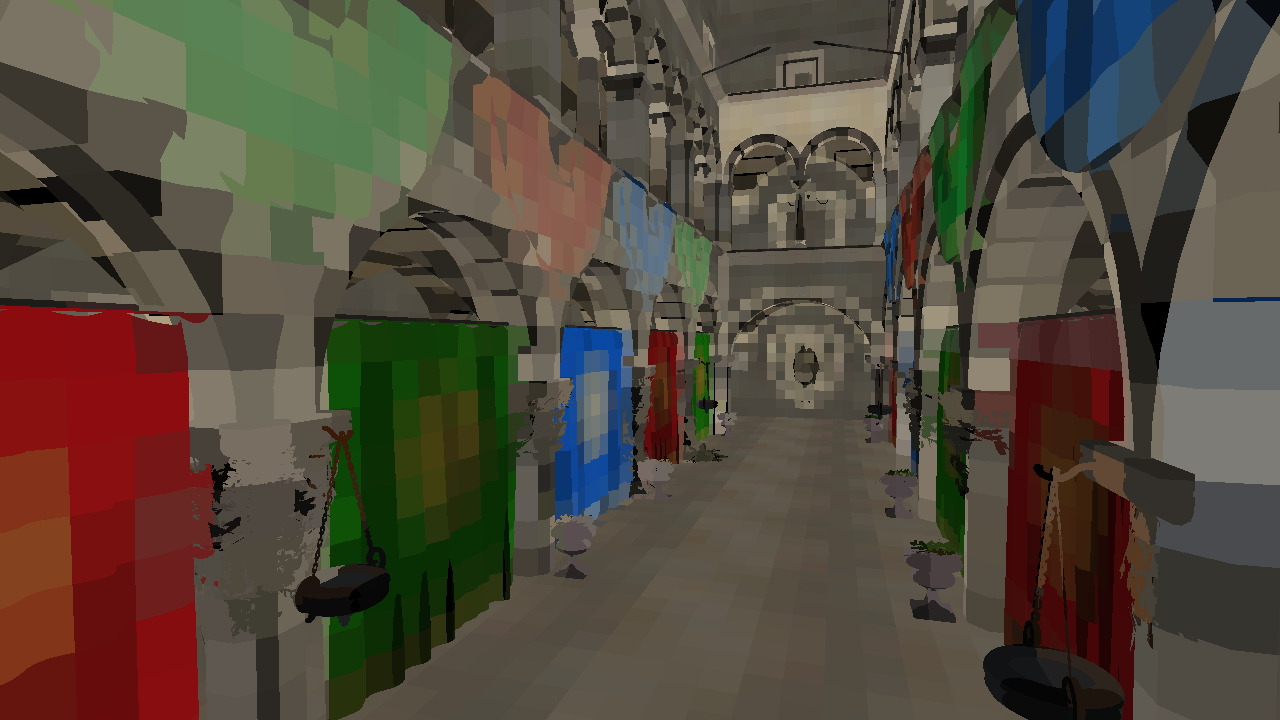
\includegraphics[width=\textwidth]{mipmap1.png}
        \caption{Level 1}
    \end{subfigure}
    \begin{subfigure}[t]{0.4\textwidth}
        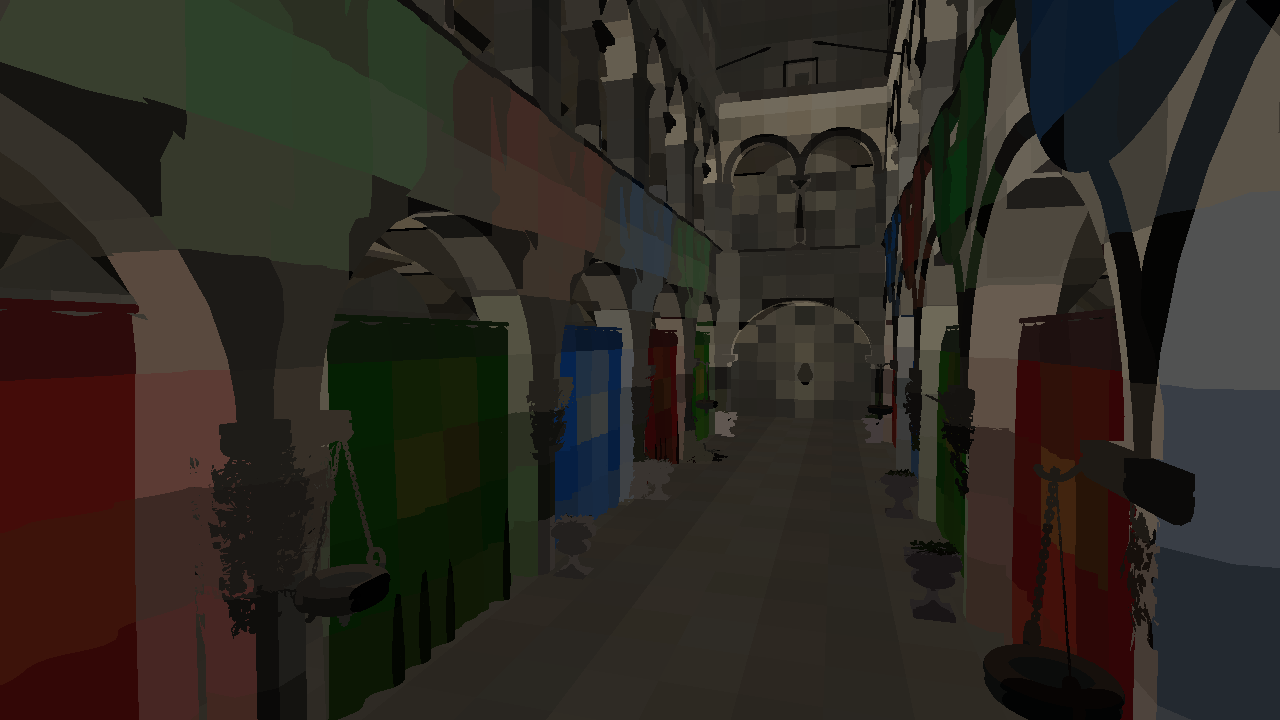
\includegraphics[width=\textwidth]{mipmap2.png}
        \caption{Level 2}
    \end{subfigure}
    ~
    \begin{subfigure}[t]{0.4\textwidth}
        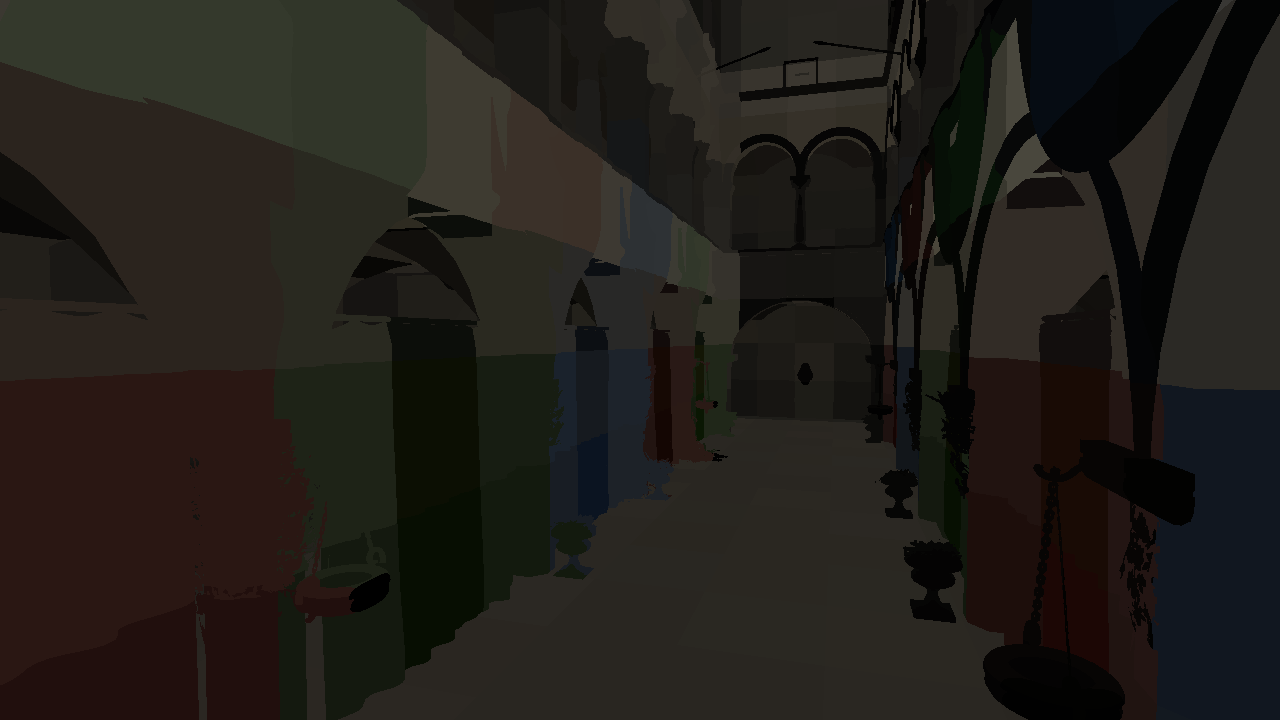
\includegraphics[width=\textwidth]{mipmap3.png}
        \caption{Level 3}
    \end{subfigure}
    \caption{The first 4 levels of the radiance texture are shown here (using \texttt{GL\_NEAREST\_MIPMAP\_NEAREST} filtering for demonstration purposes).}
    \label{fig:radiancefiltered}
\end{figure}

\section{Shading}
% TODO do i need to show code/go step by step here?
The final shading step takes all of the previously generated information and renders the scene. Direct lighting is computed from multiple lights and uses the physically based Cook-Torrance shading model~\cite{Cook:1982:RMC:357290.357293}. The classic Blinn-Phong shading model~\cite{Phong:1975:ICG:360825.360839} is also supported. Indirect lighting is computed using voxel cone tracing. Normal mapping (similar to bump mapping~\cite{Blinn:1978:SWS:965139.507101}), shadow mapping, and post processing effects also occur here. A complete outline of computing the final shaded color is shown in Algorithm~\ref{alg:finalshading}.

% TODO section  on normal mapping, shadow mapping, postprocessing?  or maybe in background?

% TODO explain UBO offsets and such? (also should this be in background?)
Two important inputs for the fragment shader are material information and light information. The material information for each fragment is provided in a struct \texttt{Material}, uploaded as a uniform buffer object, and contains color and texture information. Lights are stored as an array of struct \texttt{Light}s and contain information associated with them such as light type (e.g.\ directional or point light), position, and color. The array is uploaded as a shader storage buffer object, which allows the array to have a dynamic size queryable at shader runtime.

\begin{algorithm}
    \caption{Final Shading (performed on each rasterized fragment)}
    \label{alg:finalshading}
    \begin{algorithmic}
        \State {$directLighting = 0$}
        \For {each light in the scene}
            \State {$directLighting = directLighting + \mathrm{computeDirect}()$} \Comment{Diffuse and specular lighting}
            \If {in shadow}
                \State {$shadowFactor = \mathrm{computeShadowAmount}()$}
                \State {$directLighting = shadowFactor * directLighting$}
            \EndIf
        \EndFor
        \State {}

        \State {$indirectLighting = 0$}
        \For {each diffuse cone}
            \State {Transform cone direction to world space} \Comment{Using TBN matrix}
            \State {$color, occlusion = \mathrm{coneTrace}()$} \Comment{Perform cone tracing, resulting in a color and occlusion factor}
            \State {$indirectLighting = indirectLighting + occlusion * color$}
        \EndFor
        \State {}

        \State {$reflectedDirection = \mathrm{reflect}()$} \Comment {Compute direction of reflected ray}
        \State {$reflectColor, reflectOcclusion = \mathrm{coneTrace}()$}
        \State {$indirectLighting = indirectLighting + reflectOcclusion * reflectColor$}
        \State {}

        \State {$finalColor = directLighting + indirectLighting$}
        \State {$finalColor = finalColor / (finalColor + 1)$} \Comment{Tone map}
        \State {$finalColor = finalColor^{\frac{1}{2.2}}$} \Comment{Gamma correction}
    \end{algorithmic}
\end{algorithm}

% \missingfigure{Final rendered image with each individual contribution (direct+ diffuse indirect + specular indirect)}

\subsection{Direct Lighting}
We calculate direct lighting by iterating over each light source in the scene and summing all lighting contributions. We compute diffuse and specular lighting according to the Cook-Torrance shading model (without the ambient term, which is computed by the voxel cone tracing):
\[
    r = \sum_{i=0}^{n} l_c * (\bm{n} \cdot \bm{l}) * (d * r_d + s * r_s)
\]
where $r$ is the resulting color, $n$ is the number of lights, $l_c$ is the light color, $\bm{n}$ is the surface normal, $\bm{l}$ is the light vector, $d$ and $s$ are scaling factors, and $r_d$ and $r_s$ are the diffuse and specular components (the BRDFs). The diffuse component $r_d$ is calculated with the Lambertian model for diffuse light, which is simply $c / \pi$, where $c$ is the material's surface color. The specular component is
\[
    r_s = \frac{DGF}{\pi (\bm{n} \cdot \bm{l}) (\bm{n} \cdot \bm{v})}
\]
where $D$ is a Normal Distribution Function, $G$ is the Geometric Attenuation Fucntion, $F$ is the Fresnel term, $\bm{n}$ is the surface normal, $\bm{l}$ is the light vector, and $\bm{v}$ is the view vector. The Cook-Torrance model allows for different choices of $D$, $G$, and $F$. Our implementation uses the Trowbridge-Reitz GGX Normal Distribution Function, Smith Schlick-GGX Geometric Attenuation Function, and Schlick's approximation for the Fresnel term\footnote{These choices for $D$, $G$, and $F$ are the same as in Unreal Engine 4~\cite{karis2013real}.}:
\begin{align*}
    D(\bm{n}, \bm{h}, \alpha) &= \frac{\alpha^2}{\pi ((\bm{n} \cdot \bm{h})^2 (\alpha^2 - 1) + 1)^2} \\
    G1(\bm{n}, \bm{v}, k) &= \frac{\bm{n} \cdot \bm{v}}{(\bm{n} \cdot \bm{v}) (1 - k) + k} \\
    G(\bm{n}, \bm{v}, \bm{l}, \bm{k}) &= G1(\bm{n}, \bm{v}, k) G1(\bm{n}, \bm{l}, k) \\
    F &= F0 + (1 - F0) (1 - \cos \theta)^5 \\
\end{align*}
where $\alpha$ is material roughness, $\bm{h}$ is the half vector, $k = \frac{(\alpha + 1)^2}{8}$, $\theta$ is the angle between $\bm{h}$ and $\bm{v}$, and F0, the surface reflection at zero incidence, is 0.04 for dielectrics and the surface albedo for metals\footnote{This is not completely physically accurate but is a good and fast approximation.}.

% TODO definitely gonna want some pictures
% TODO present integral as going backwards? (want integral -> inf many rays -> break into discrete chunks w/ weights)
\subsection{Indirect Lighting (Voxel Cone Tracing)}
To compute the indirect lighting at a given point, we perform voxel cone tracing. Recall that to compute indirect light we are effectively approximating a surface integral over a hemisphere. With voxel cone tracing, this integral is reduced to summing the contributions of several cones, each of which are defined by a direction and cone angle\footnote{Note that as the cone angle approaches zero we effectively have a ray. In fact, the main difference between classic raymarching and cone tracing is the cone angle (which is used to determine which level of the filtered radiance to sample from).}. To compute the integral perfectly would require infinitely many cones. Instead, we use six cones: five for diffuse light and one for a specular highlight\footnote{The number of cones and their associated directions and angles are determined experimentally.}.

% TODO should either explain vct in related works or right here before detailing cone properties
% TODO multiple cones + directions, weights and math supporting it
% TODO FILL IN APERTURE (from vct settings) AND ANGLE
For the diffuse cones we chose an aperture of $45^\circ$ with one cone oriented in the direction of the surface normal and the others evenly distributed around the normal and tilted up at an angle of $45^\circ$. We also assign weights to each cone based on a uniform distribution. Note that in order to compute the orientation of each cone in world space we must multiply the chosen cone directions by the TBN matrix, since the cone directions are defined in tangent space. To get the final diffuse contribution, the cone tracing is performed for each cone and the values are weighted and summed appropriately.

% TODO make sure to define these somewhere
The specular cone is oriented in the direction of the reflection vector, which is calculated as $-\bm{v} - 2 * (\bm{n} \cdot -\bm{v}) * \bm{n}$, or by using the GLSL function \texttt{reflect()}. The aperture is derived from the material's roughness according to the following formula\footnote{Determined experimentally.}: $0.1 * \pi * roughness$.

% \missingfigure{Show hemisphere with the cones used}

% TODO place this somewhere...
% TODO  add math n shit yo
The radiance texture is sampled at varying levels of detail in order to approximate the amount of indirect light at that point. At it's core, voxel cone tracing is raymarching through a mipmapped texture. In order to determine which miplevel to sample from, the idea of cone tracing is introduced. Instead of having a simple ray, we imagine a cone with a particular aperture (angle). The cone's height is analagous to a ray's length and the size (diameter) of the cone's base grows as the height increases. We can then map the diameter to a level of detail.

Combining this all together, we sample from the radiance texture at a level of detail related to the height of the cone at our sampling point. In this way, samples close to the start of the cone come from higher detailed data and samples far from the start come from lower detailed data. This allows the voxel cone tracing to gather both high frequency and low frequency details of the indirect light.

% TODO go over all the vct settings
The implementation of a single cone tracing instance is done entirely within a fragment shader. The main inputs are the radiance texture, the position to start tracing from, and the direction in which to trace. There are also several configurable parameters that influence the cone tracing. We have \texttt{steps}, the maximum number of samples to take; \texttt{bias}, the initial offset from the starting position (in order to avoid self illumination); \texttt{coneAngle}, the angle of the cone; \texttt{coneHeight}, the starting height of the cone; and \texttt{lodOffset}, a constant offset used when determining the level of the radiance texture to sample from. Also, since the cone tracing is performed in texture space, a \texttt{scale} is applied to normalized direction vectors. For each step, the cone's radius is computed from the cone's height and angle. From this, we compute the level of detail to sample from. After getting the sample color and alpha value a forward blending scheme is used. Finally, the cone's height is increased for the next iteration of the loop. The complete shader code for cone tracing is shown in Listing~\ref{lst:vct}. The lighting contribution from the indirect light (both diffuse and specular) is displayed in Figure~\ref{fig:debugindirect} and the occlusion values are displayed in Figure~\ref{fig:debugocclusion}.

\begin{lstlisting}[caption={Shader function for performing voxel cone tracing.},label={lst:vct}]
vec4 traceCone(sampler3D voxelTexture, vec3 position, vec3 normal, vec3 direction, int steps, float bias, float coneAngle, float coneHeight, float lodOffset)
{
    vec3 color = vec3(0);
    float alpha = 0;

    float scale = 1.0 / voxelDim;
    vec3 start = position + bias * normal * scale;
    for (int i = 0; i < steps && alpha < 0.95; i++) {
        float coneRadius = coneHeight * tan(coneAngle / 2.0);
        float lod = log2(max(1.0, 2 * coneRadius));
        vec3 samplePosition = start + coneHeight * direction * scale;

        vec4 sampleColor = textureLod(voxelTexture, samplePosition, lod + lodOffset);
        float a = 1 - alpha;
        color += sampleColor.rgb * a;
        alpha += a * sampleColor.a;
        coneHeight += coneRadius;
    }

    return vec4(color, alpha);
}
\end{lstlisting}

% \begin{algorithm}
%     \caption{Voxel Cone Tracing}
%     \label{alg:voxelconetracing}
%     \begin{algorithmic}
%         \Procedure{TODO}{}
%         \EndProcedure
%     \end{algorithmic}
% \end{algorithm}

\begin{figure}[h!]
\centering
    \begin{subfigure}[t]{\textwidth}
        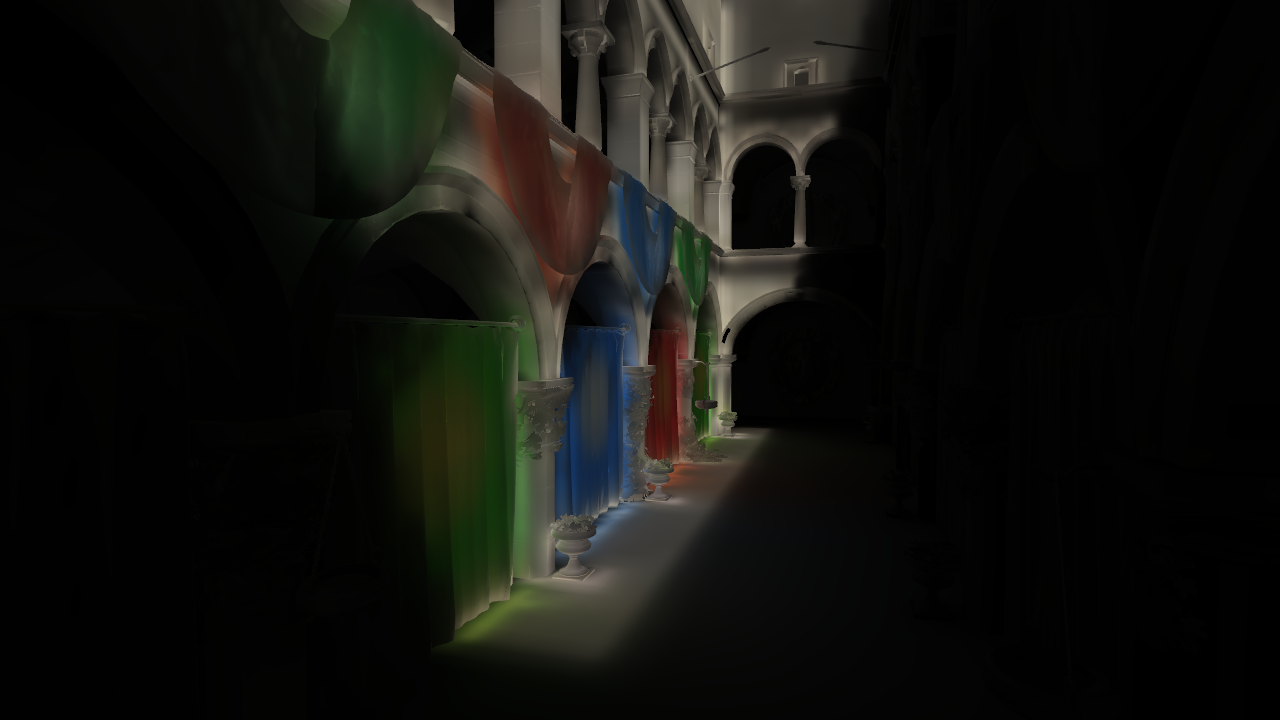
\includegraphics[width=\textwidth]{debugIndirect_noOcclusion.png}
        \caption{Diffuse indirect light}
    \end{subfigure}
    \begin{subfigure}[t]{\textwidth}
        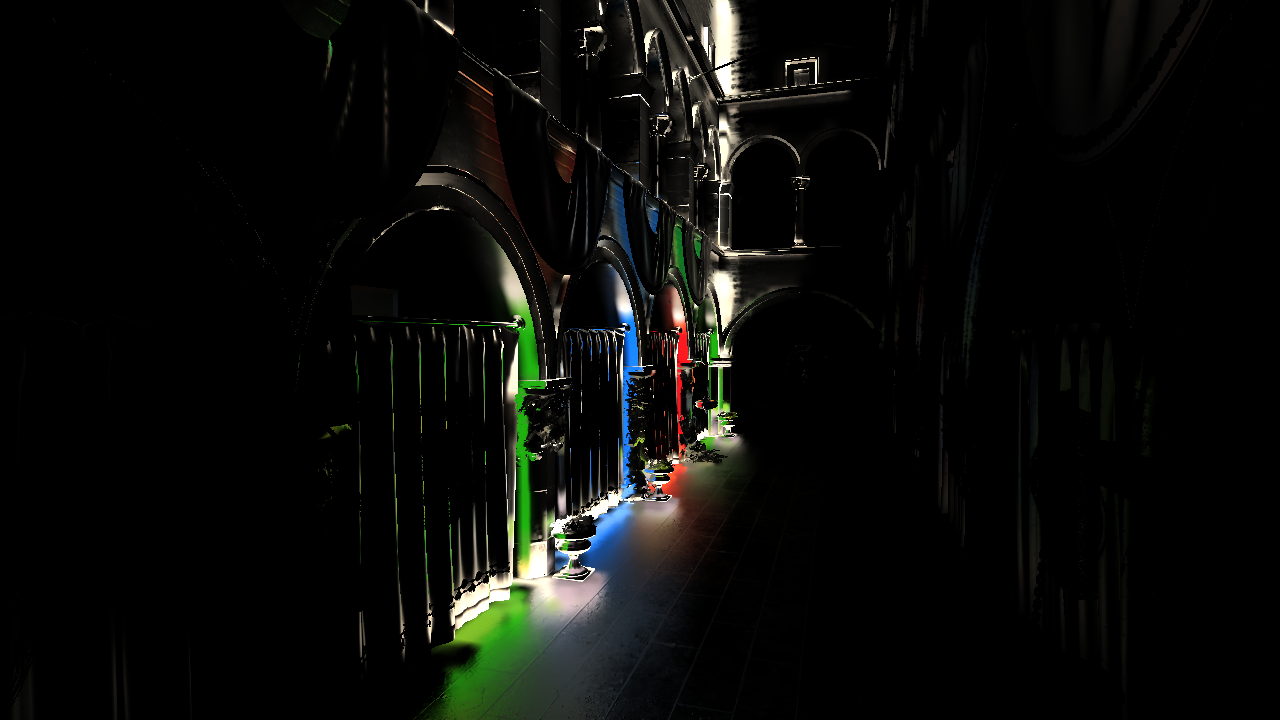
\includegraphics[width=\textwidth]{debugReflections.png}    % TODO multiplied by occlusion?
        \caption{Specular indirect light}
    \end{subfigure}
    \caption{The diffuse and specular contributions from cone tracing (before multiplying by occlusion).}
    \label{fig:debugindirect}
\end{figure}

\begin{figure}[h!]
\centering
    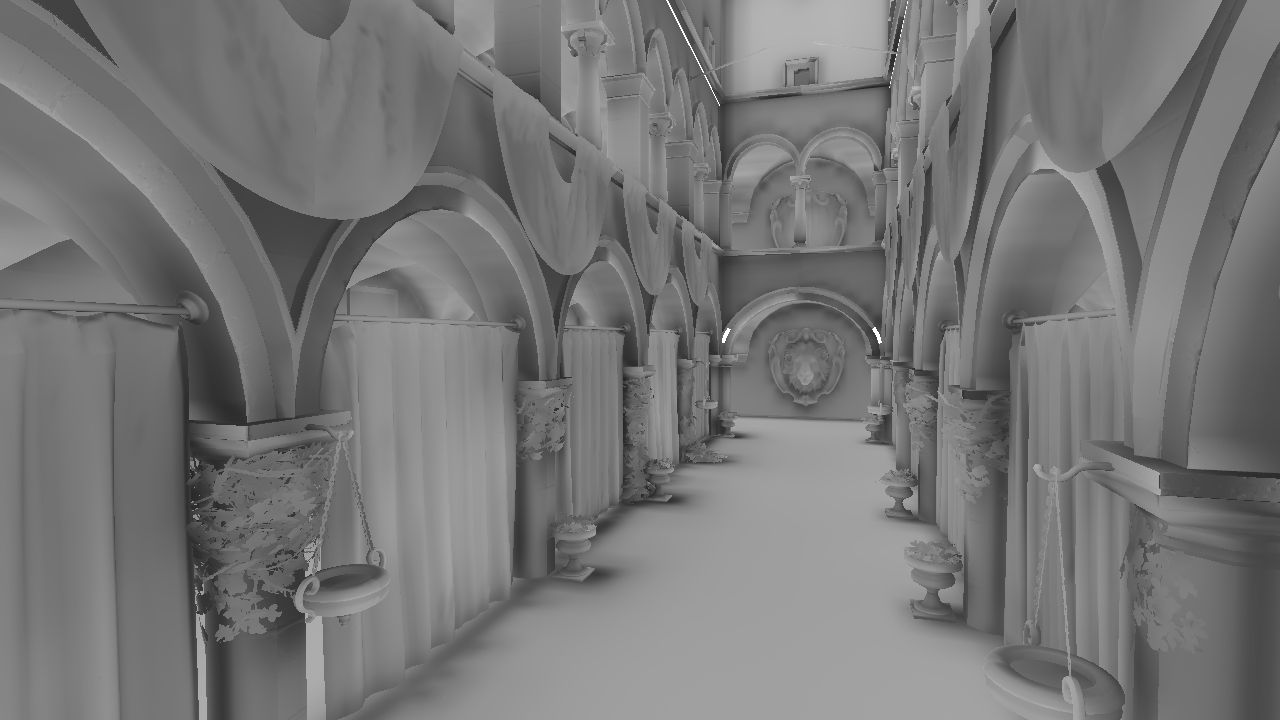
\includegraphics[width=\textwidth]{debugOcclusion.png}
    \caption{Occlusion values resulting from voxel cone tracing. The occlusion is multiplied with the cone traced lighting in order to account for occlusion of nearby objects (i.e.\ voxel based ambient occlusion).}
    \label{fig:debugocclusion}
\end{figure}

\section{Voxel Warping}
% TODO deriving spline, why need constraints, increasing viewport resolution
The goal of voxel warping is to vary the density of the voxel resolution according to some metric. This effectively increases the detail of the voxelization, leading to better global illumination. We present two different approaches for voxel warping: warp functions and perspective warping.

\subsection{Using a Warp Function}
Previously, voxel positions were determined linearly from their position inside the voxel volume to a position in the voxel texture. This approach takes that linear position and applies a mapping to it to find the final position inside the voxel texture. With an appropriate warping function, the voxel density can be modified. For this approach, the warping function's job is to increase detail near the camera and then smoothly fall off for objects further away.

\subsubsection{Linear Warp Function}
Recall from voxelization that in order to determine the location in the voxel texture for a given fragment we perform a linear mapping from world space to image space. As an intermediate step, we have the voxel position in texture space (in the range $[0, 1]$). Thus, for example, if the position along the $y$ axis is 0 it will go into the bottom of the voxel texture and if 1 will go into the top part of the voxel texture. Now, consider mapping the coordinate in texture space to so-called warp space, which is also in the range $[0, 1]$. Without any modifications, this is a straight line with a slope of 1, representing a linear `warping' function. If we let $w_{linear}: [0, 1] \rightarrow [0, 1]$ be the warping function and $x \in [0, 1]$ be the coordinate in texture space then we have $w_{linear}(x) = x$. Of course, this warping function does not do anything useful. For that, we need a different, nonlinear, warping function.

\subsubsection{Nonlinear Warping}
Consider the function $w_{logistic}(x) = \frac{1}{1 + e^{-x}}$ (a basic logistic function, a type of ``S''-shaped curve). Notice how as $x$ approaches 0 or 1 the slope decreases and in the middle the slope is greater than one. If we draw lines up and over from the curve for $x = 0.4$ and $x = 0.6$ we see that the range of $w_{logistic}(x)$ is greater than that of $w_{linear}(x)$. In other words, the positions within those particular $x$ values `take up more space' in the voxel texture. Likewise, towards the ends, the slope decreases towards zero and thus takes up less space. This achieves the goal of varying the voxel density resolution according to a simple function. We also see that the slope, $w'(x)$, represents the voxel density: if $w'(x) = 1$, the density is the same as the linear mapping; if $w'(x) > 1$, the density is greater than the linear mapping; if $w'(x) < 1$, the density is less than the linear mapping.
% TODO lots of pictures, show  functions and lines; start off with cubic instead?

The ideal warping function increases voxel density near the camera and decreases voxel density further away. The logistic function provided does this\footnote{The camera is at the center of the voxel grid, so it corresponds to $x = 0.5$ in the warping function.}, however there are some issues. Recall from the Voxelization section that the scene is rendered with a viewport of dimensions equal to that of the voxel texture. The discretized fragment positions will therefore all be in step sizes corresponding to this viewport resolution. When the warp function is applied where $w'(x) > 1$, we can run into issues where adjacent fragments will `skip' a position in the voxel texture. In essence, the voxel fragments are not generated with fine enough resolution to smoothly transition after being warped \footnote{This is similar to the concept of the Nyquist Frequency, where we are not sampling the signal at a high enough rate}. To resolve this, the scene must be voxelized with a viewport resolution scaled by the maximum derivative of $w(x)$. In design terms, this means choosing a warping function with a steep slope will result in needing to voxelize the scene with a larger viewport resolution, which can hurt performance. Figure~\ref{fig:voxelcracks} demonstrates this issue.

\begin{figure}[h!]
    \centering
    \begin{subfigure}[t]{\textwidth}
        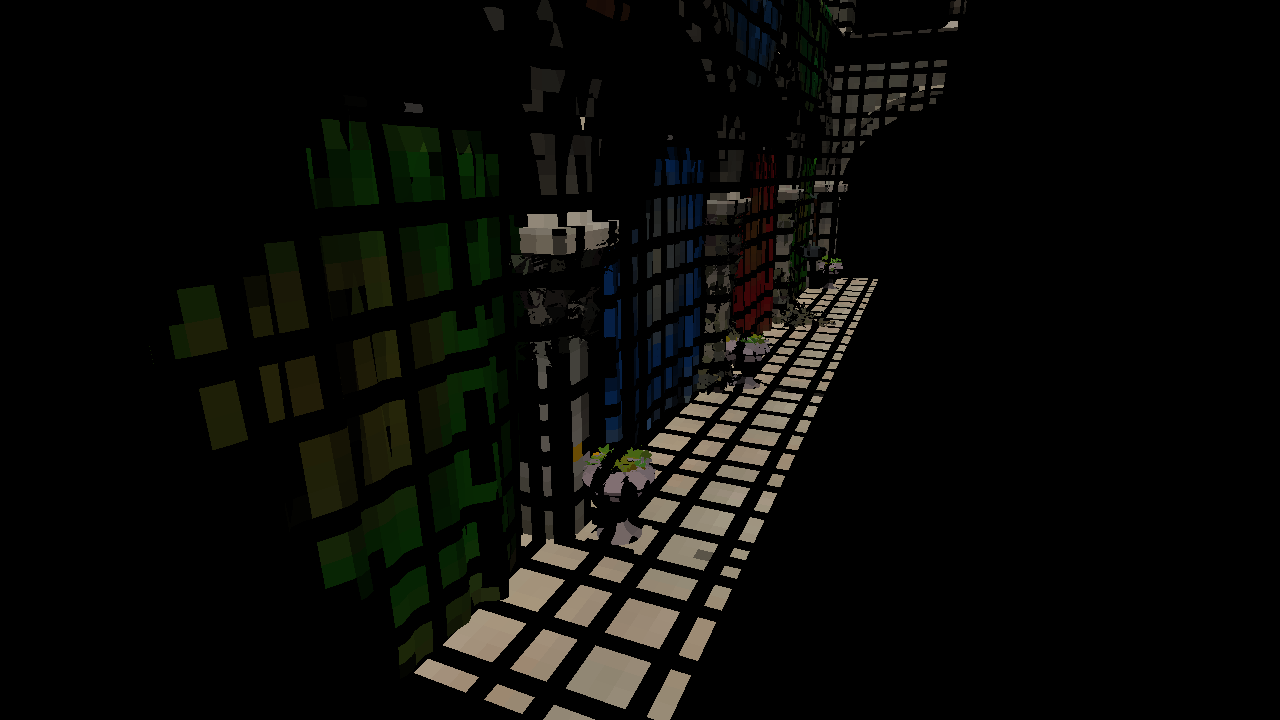
\includegraphics[width=\textwidth]{voxelwarp_cracks.png}
    \end{subfigure}
    \begin{subfigure}[t]{\textwidth}
        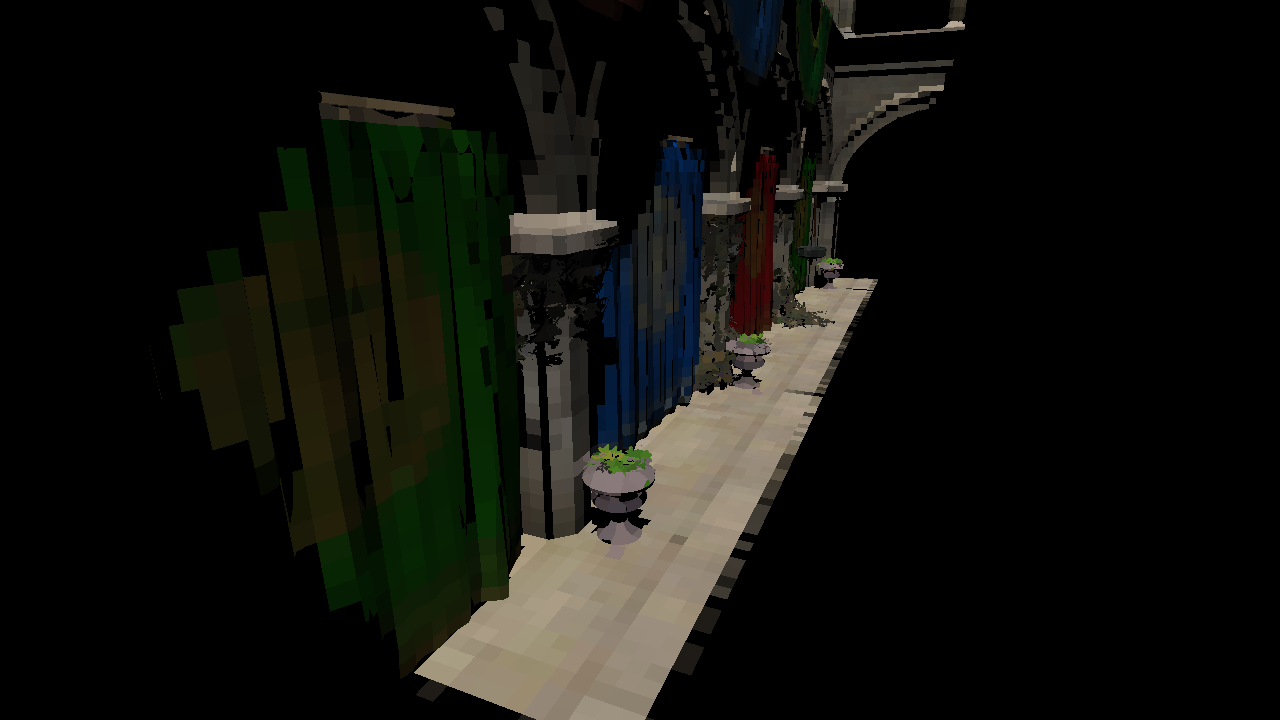
\includegraphics[width=\textwidth]{voxelwarp_nocracks.png}
    \end{subfigure}
    \caption{Cracks in the voxels caused by higher voxel density (left) and filling the holes by voxelizing with a higher resolution (right).}
    \label{fig:voxelcracks}
\end{figure}

Using the logistic function as the warping function also has another issue: the slope at the ends approaches zero. This leads to a large portion of the voxelized region ending up in relatively few voxels, which diminishes the accuracy of the voxelization greatly. % TODO show this
Instead, we want to place a lower bound on $w'(x)$. The solution to this is to use a cubic spline, i.e.\ $w(x) = a + bx + cx^2 + dx^3$. Then, with $\alpha$ as the desired end slope, we use the constraints $w(0) = 0, w(1) = 1, \text{ and } w'(0) = w'(1) = \alpha$ and solve for the variables $a$, $b$, $c$, and $d$. This gives the warping function: $w(x) = \alpha x + (3 - 3 \alpha) x^2 + (2 \alpha - 2) x^3$. For our implementation, $\alpha = 0.25$.

% TODO imply that 0.5 is close to camera? idk
% TODO go over how this doesnt mess up voxel cone tracing or filtering and stuff
% TODO horner's method?

% \subsection{Warp Textures}  % TODO ???

\subsection{Perspective Warping}
The other method of warping implemented is based on perspective projection. Recall that when transforming coordinates from view space to clip space we use a projection matrix. To emulate the visual effect of distant objects appearing smaller, a perspective projection matrix applies a scaling factor to any transformed position coordinate. This scaling effectively causes distant objects to occupy less area in screen space of the final rendered image. Similarly, for our perspective warping, we use a perspective matrix to manipulate the final voxel position.

To determine the voxel position from a position in world space, we apply both a perspective projection and view matrix. This results in a point in NDC corresponding to its position within the view frustum\footnote{We also must linearize the depth (z) component of the position, as a perspective projection causes the depth to be logarithmic.}. This value is then shifted and scaled to be in texture space, which is the voxel position.

% TODO do i need this?
\section{Miscellaneous}
\subsection{Depth Prepass}
With voxel cone tracing, each fragment shader invocation is quite expensive. If we have overlapping objects in the scene then fragments will be shaded for each pixel, but only one will be the final color. To ensure we only shade the final fragment, we have a prepass which rasterizes the scene and only writes the depth value. This operation is extremely quick. Now, the depth buffer contains only the depth of the fragment that will end up on the screen. When the full shading pass is performed all fragments that fail the depth test can be immediately discarded, avoiding the expensive voxel cone tracing\footnote{This technique is only needed for a forward rendering engine: for a deferred rendering engine the final depth values are calculated when generating the G-buffer (geometry buffer).}.
% TODO give before/after improvement

% \subsection{Compressed Textures with Pregenerated Mipmaps}
% TODO ?

\subsection{Temporal Filtering}     % TODO ???
Typically the radiance texture is cleared completely at the beginning of each frame. Due to the discrete nature of the voxel grid, moving objects and lights can cause temporal artifacts (flickering) as the voxels are updated. These artifacts can be improved by incorporating previous radiance values into the current frame's radiance. To do this, we can blend some factor of a voxel's previous radiance value with its new value\footnote{This factor is configurable at runtime.}.

% \subsection{Voxel Hole Filling}     % TODO ??? (radianceDilate,voxelizeDilate,voxelFillHoles)


% TODO custom filtering, try raymarching optimizations from nvidia blog